\documentclass[11pt]{article}

\usepackage[margin=1in]{geometry}
\usepackage{setspace}
\onehalfspacing
\usepackage{graphicx}
\graphicspath{report_images/}

% DOCUMENT INFORMATION =================================================
\title {ECEN 429: Introduction to Digital Systems Design Laboratory \\ North Carolina Agricultural and Technical State University \\ Department of Electrical and Computer Engineering} % Declare Title
\author{Reporter: Chris Cannon \\ \and Partner: Nikiyah Beaulah} % Declare authors
\date{February 1, 2018}
% ======================================================================

\begin{document}

\maketitle % Render Title, Author, and Date

\begin{center}
Lab	1
\end{center}

\pagebreak

\section{Introduction}
For this first lab our task was to familiarize ourselves with Xilinx Vivado Design Suite and the Digilent Basys3 FPGA Development Board that is used in this lab. During these tasks we learned how to configure the settings on Vivado for our board and how to load a program to the board. We also have three programming assignments for this lab. The first assignment was to write a simple VHDL program using an AND gate with two inputs and one output. The second assignment was to write a VHDL program using the car alarm example which that we derived in class. Our car alarm consists of 3 inputs using switches and 2 outputs using LED lights.  The third assignment was to create our own design implementation and write a VHDL program using only 4 inputs and 3 outputs. For our third assignment, we elected to build an adder for two 2-bit numbers. Upon successfully completing this lab, we will be able to work comfortable translating our circuit designs and VHDL code to a Vivado project and implement it on the Basys3 board.

\section{Background, Design Solution, and Results}
\subsection{Problem 1: 2-bit AND Gate}

The inputs for this problem are named 'A' and 'B' and the output is named 'C'.


\begin{table}[h]
\begin{center}
	\begin{tabular}{| l | l | l |}
		\hline
		Bit & Label & Address\\ \hline
		A & Switch 1 & V16\\ \hline
		B & Switch 7 & W13\\ \hline
		C & LED 3 & V19\\ \hline
	\end{tabular}
	\caption{\label{tab:table-name}Input and output bit specifications for problem 1.}
\end{center}
\end{table}

These inputs and outputs will interact according to the properties of an AND gate, shown in the truth table below.

\begin{table}[h]
\begin{center}
	\begin{tabular}{| l | l | l |}
		\hline
		A & B & C \\ \hline
		0 & 0 & 0 \\ \hline
		0 & 1 & 0 \\ \hline
		1 & 0 & 0 \\ \hline
		1 & 1 & 1 \\ \hline
	\end{tabular}
	\caption{\label{tab:table-name}Truth Table for Problem 1.}
\end{center}	
\end{table}



\subsection{Problem 2: Car Alarm}

Problem 2 referenced a car alarm system designed in class. The car alarm is made up of two sensors, a vibration sensor ('V') and a door sensor ('D'). The system is considered "active" when the master switch ('M') is activated. The car alarm has one output, an alarm siren ('S'). The logical circuit diagram for this is noted below.
\begin{figure}[h]
	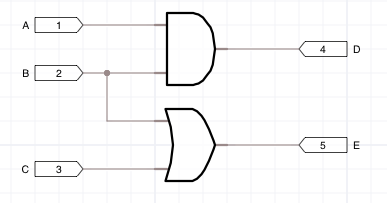
\includegraphics[width=\textwidth]{report_images/img1}
	\caption{\label{fig:figure-name}Circuit diagram for car alarm.}
\end{figure}

The circuit if Figure 1 above translates to the following truth table:

\begin{table}[h]
\begin{center}
	\begin{tabular}{| l | l | l | l |}
	\hline
	D & V & M & S \\ \hline
	0 & 0 & 0 & 0 \\ \hline
	0 & 0 & 1 & 0 \\ \hline
	0 & 1 & 0 & 0 \\ \hline	
	\end{tabular}
	\caption{\label{tab:table-name}Truth table for the car alarm.}
\end{center}
\end{table}


The given map for the input and output bits told us where we should assign each bit from our system.

\begin{table}[h]
\begin{center}
	\begin{tabular}{| l | l | l |}
		\hline
		Bit & Label & Address \\ \hline
		D & Button L & W19 \\ \hline
		V & Switch 15 & R2 \\ \hline
		M & Button R & T17 \\ \hline
		D & LED 7 & V19 \\ \hline
		E & LED 6 & U14 \\ \hline
	\end{tabular}
	\caption{\label{tab:table-name}Input and output bit specification for car alarm.}
\end{center}	
\end{table}


\subsection{Problem 3: Design Our Own Circuit}


\end{document}
